\documentclass[parskip]{scrartcl}
\usepackage[margin=15mm]{geometry}
\usepackage{tikz}
\usetikzlibrary{snakes,decorations.pathreplacing}

\newcommand{\flux}{yellow!75!gray}
\newcommand{\rightcoil}{green!85!gray}
\pgfmathsetmacro{\coilStart}{7}
\pgfmathsetmacro{\coilEnd}{8}

\begin{document}
%~~~~~~~~~~~~~~~~~~~~~~~~~~~~~~~~~~~~~~~~
% ELEC 467 Electric Machines and Transformers
% AC Electromagnetic Relay Diagram
% Written by Sze "Ron" Chau, October 2014
%
%~~~~~~~~~~~~~~~~~~~~~~~~~~~~~~~~~~~~~~~~
% first time using Tikz - while working Halloween
% overnight at Children's Hospital and my patient codes.
% add to the fact that I HAVE NO IDEA WHAT I'M DOING
% this might read like super spaghetti
%~~~~~~~~~~~~~~~~~~~~~~~~~~~~~~~~~~~~~~~~

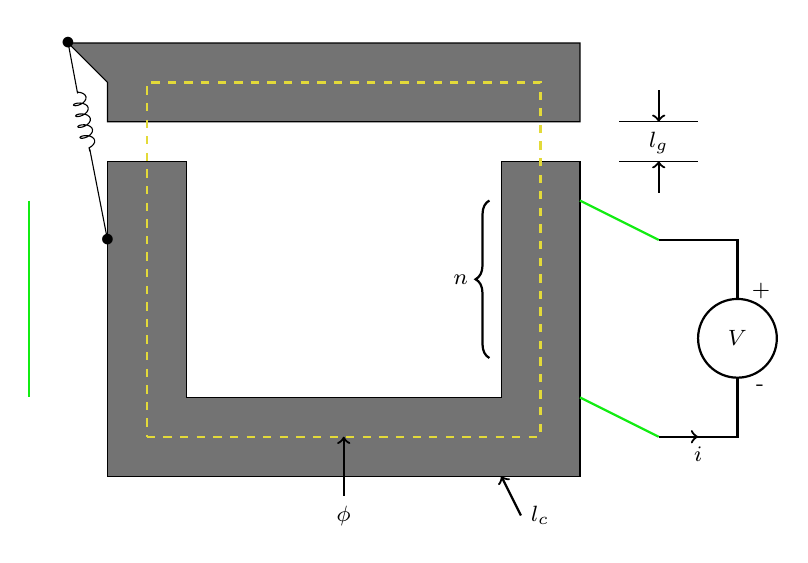
\begin{tikzpicture}

% relay
\filldraw[fill=gray!90!black, draw=black](2,1) -- (8,1) --
    (8,5) -- (7,5) -- (7,2) -- (3,2) -- (3,5) -- (2,5) -- cycle;
\filldraw[fill=gray!90!black, draw=black](2,5.5) -- (8,5.5) --
    (8,6.5) -- (1.5,6.5) -- (2,6) -- cycle;

% spring
\node(top) at (1.5,6.5){$\bullet$};
\node(bottom) at (2,4){$\bullet$};
\draw(1.5,6.5) -- (1.62,5.86);
\draw(1.775,5.15) -- (2,4);
\node(springTop) at (1.6,6){};
\node(springBottom) at (1.8,5){};
\draw[snake=coil,segment length=4pt](springTop) -- (springBottom);

% flux lines
\draw[thick,dashed,draw=\flux](2.5,1.5) -- (7.5,1.5) --
    (7.5,6) -- (2.5,6) -- cycle;
\draw[thick,->](5,0.75) node[below]{\footnotesize$\phi$} --
    (5,1.5);

% lengths of air gap and core
\draw(8.5,5) -- (9.5,5);
\draw(8.5,5.5) -- (9.5,5.5);
\draw[thick,->](9,5.9) -- (9,5.5)
    node[below]{\footnotesize$l_{g}$};
\draw[thick,->](9,4.6) -- (9,5);
\draw[thick,->](7.25,0.5)
    node[right]{\footnotesize$l_{c}$} -- (7,1);

% coils
\foreach \leftY in {2.5,3,3.5,4,4.5}
{
    \draw[thick,\rightcoil](\coilStart,\leftY) --
    (\coilEnd,\leftY-0.5);
}
\draw[thick,\rightcoil](8,4.5) -- (9,4);
\draw[thick,\rightcoil](8,2) -- (9,1.5);
\draw[thick,decorate,decoration={brace,amplitude=5pt}]
    (6.85,2.5) -- (6.85,4.5) node[midway, left=4pt] {\footnotesize$n$};
    
% power supply
\draw[thick](9,4) -- (10,4) -- (10,3.25) 
    node[above=3pt,right=1.5pt]{\footnotesize+};
\draw[thick](9,1.5) -- (10,1.5) -- (10,2.25)
    node[below=3pt,right=3pt]{\footnotesize-};
\draw[thick](10,2.75) circle (.5) 
    node {\footnotesize$V$};
\draw[thick,->](9,1.5) -- (9.5,1.5) 
    node[below]{\footnotesize$i$};

\end{tikzpicture}

\end{document}